\documentclass[10pt,a4paper]{article}

\usepackage{amsmath}
\usepackage{amsfonts}
\usepackage{amssymb}
\usepackage{booktabs}
\usepackage[margin=2.5cm]{geometry}
\usepackage{graphicx}
\usepackage{chngpage}

\author{B00902031 Kevin Tsai, B00902107 Suhorng You}
\title{CN HW2 report}

\begin{document}

\maketitle

\section{Introduction}
    In this homework, we have implemented a modification of Go-Back-N protocol with partially realized connection management. The sender transmits $8$ packets without waiting for acknowledgements of each packet. To simplify the design, in each connection, data to be sent is given to the sender as a stream, and \texttt{rdt\_send} is automatically invoked by the sender when the window is empty to refill the window by data from the stream. Similar changes is made to the receiver. When called, the receiver blocks and wait until a transmission came, and it automatically allocates memory to store data, returns when all data has arrived.

    We also add connection termination control to both sender and receiver to handle when to end a transmission. The connection termination phase is drawn from that of the TCP's, except that we use a three-way handshake since the connection is unidirectional.

    ``make'' compiles two binary files: ``sender'' and ``receiver.'' Start receiver at the target computer, and then execute sender to send the file. The file sent will be saved at the working directory of sender, which is normally the directory sender is in. Filename and file permissions are preserved during the transmission. If there already exists a file with the same name, the transmission will be terminated. Sender closes after the transmission, but the receiver continues to wait for the next file until it is aborted (maybe by \texttt{\^{}C}).

    Command line arguments is as follows:
\begin{verbatim}
$ make                                                                    build targets
$ make clean                                             clean targets and object files
$ ./receiver LISTEN_PORT                     receive files, waiting at port LISTEN_PORT
$ ./sender TARGET_HOSTNAME TARGET_IP FILENAME                                 send file
\end{verbatim}

    Transferring multiple files simultaneously is not supported, however.
\section{Unreliable Data Transfer Layer}
    This layer simply uses UDP to transfer data. This layer provides functions to open UDP sockets, to send packages to and receives packages from the socket, and to close the socket. The receive and send functions are both blocking, but the receive function only waits for a limited time which can be set by the function caller and is $0.5$ seconds by default. This layer also provides an additional function that clears the socket buffer in case that there are any redundant packages left in the socket.

\section{Reliable Data Transfer Layer}
\subsection{Packet Format}
    The size of packets varies from $9$ bytes to $256$ bytes. The first byte of the packet specifies the size of the following data, that is, $8$ bytes plus the length of the content. It is followed by a $4$-byte unsigned integer sequence number, and a $4$-byte unsigned int CRC-32 checksum. The rest are the actual data that we want to transfer, whose length could be from $1$ byte to $247$ bytes.

\begin{center}
    \begin{adjustwidth}{-.7cm}{2cm} % adjust the left-bound -0.7cm and right-bound 2cm
        \begin{tabular}{lcc}
            Entry Name & Size (bytes) & Interpretation \\%& Type & Meaning\\
                \hline
            packet size & $1$ &  size of the packet (exclusive of this entry)\\ 
            sequence number & $4$ & sequence number of the packet\\
            checksum & $4$ & the CRC-32 checksum of the whole package, with this entry treated as zero\\
            data & $1$-$247$ & the data being transferred\\
        \end{tabular}
    \end{adjustwidth}
\end{center}
    
\subsection{Receiver and Sender FSM}
    \begin{center}
        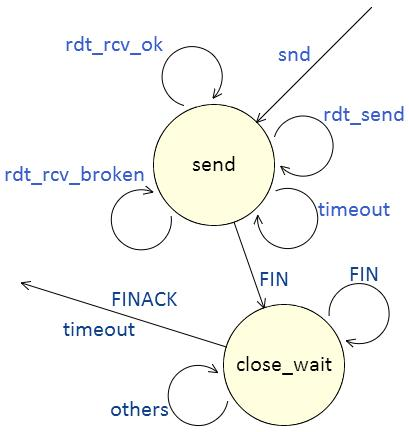
\includegraphics[scale=0.7]{fsmsnd.jpg}
        \; \; \;
        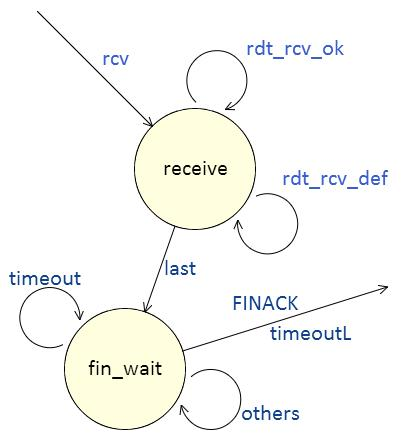
\includegraphics[scale=0.7]{fsmrcv.jpg}\\
        {\small Fig.1 \; The state diagram of the sender and receiver; Go-Back-N with extended FSM}
    \end{center}
    Figure 1 is the diagram of the sender and the receiver, respectively. The details are described below. 

    Roughly speaking, when calling the sender, it first clears the buffer, sends data, and wait. If timeout, the packets in the window are resent. If received ACK, the sender slides the window to the right until \texttt{base} touches received sequence number, i.e. only those packets that haven't been ACKed are left. Both corrupted packets and out-of-range ACKs are simply ignored. If FIN, which is the same as the ACK of the last packet, is received, the sender enters termination phase to close the connection.

    When calling the receiver, it waits for data to come, and accepts only the packet with sequence number equals \texttt{expseq}. If the received packet is not accepted, it simply throws it away and resend previous ACK (or ACK-INIT, is no packet ever accepted). When regarded data in the packets as a stream, the first 4 bytes specify the total length, and hence the receiver can judge when should the connection be closed. Upon the last packet is accepted, the receiver sends FIN to the sender to require the termination of the connection.

    The three-way termination phase is initiated by the receiver. The receiver first send FIN to the sender and waits for FINACK. If the sender sends too many incorrect replies or the timer time-out, the receiver will resend FIN. As soon as the receiver received FINACK, it sends the last FINACK to sender and returns to the caller, regardless the FINACK is correctly sent to the sender or not. However, after 15 seconds of wait, the receiver still exits no matter FINACK  has ever been received or not. If the sender receives FINACK, the connection is the closed. If FINACK is lost, the connection still terminates after timeout (30s).
\begin{verbatim}
snd            rcv
|    <---FIN---  |    FIN == last packet's ACK
| \              |
|  --FINACK-->  -|
|                /
|    --FINACK----
|   /
| <-
\end{verbatim}
    \subsubsection{Sender}
    \begin{enumerate}
    	\item \texttt{snd}: initial data stream, \texttt{base}, \texttt{nxtseq} (the window); empty socket buffer; invoke \texttt{rdt\_send}
        \item \texttt{rdt\_send}: fill window by data until full; send packets
        \item \texttt{rdt\_rcv\_ok}: slide the window if $\texttt{seq}$ is correct, otherwise do nothing
        \item \texttt{rdt\_rcv\_broken}: pretending that nothing happens
        \item \texttt{timeout}: resend packets in the window
        \item \texttt{send::FIN}: send FINACK
        \item \texttt{others}: ignore
        \item \texttt{close\_wait::FIN}: send FINACK
        \item \texttt{FINACK}, \texttt{close\_wait::timeout}:
    \end{enumerate}
    \subsubsection{Receiver}
    \begin{enumerate}
        \item \texttt{rcv}: empty socket buffer; initial default reply (ACK-INIT)
        \item \texttt{rdt\_rcv\_ok}: make new ACK reply; send reply, increase $\texttt{expseq}$ by 1. If this is the very first packet the receiver ever received, read 4 bytes stream length and initial the data stream. If this is the last packet to be received, send FIN instead and go to \texttt{last}.
        \item \texttt{rdt\_rcv\_def}: send previously made reply
        \item \texttt{last}: (should send FIN)
        \item \texttt{timeout}: resend FIN
        \item \texttt{others}: ignore; but if too many unexpected packet arrived, resend FIN.
        \item \texttt{FINACK}, \texttt{timeoutL}: for \texttt{FINACK}, send FINACK and exit. for \texttt{timeoutL}, exit.
    \end{enumerate}
\subsection{Protocol}
\section{Loss and error solving}
    \subsection{Packet loss solving}
        
    \subsection{Packet error solving}
        There is a checksum in every packet sent. When received, the program checks if the checksum in the package is correct. Corrupted packets are ignored. The use of CRC-32 which is based on cyclic error-checking codes guarantees low error rate.

\section{Application Layer}
    Sender and receiver calls the RDT (reliable data transfer) layer multiple times to send a file. More precisely, the sender sends four things in order: the file's name, the file's permission, the file's size, and at last the file's content. The first three items are sent in one call, and the last one may be sent in many calls. The receiver receives the four things in order, and creates the file after it gets the file's size.

\section{Extra work}
    In addition of rdt3.0, we also implemented Go-Back-N and connection-finishing, which both make the sending process stabler. Connection-finishing is implemented by sending FIN packages and using three-way handshake. The details are described above in the ``Reliable Data Transfer Layer'' section.


    Also, the file's name and permissions are preserved under transmission.
\section{Snapshots}
\end{document}